\setcounter{chapter}{4}
\chapter{Implementation}
\label{ch:implementation}

This chapter documents the implementation of each major module in SmartHire, covering purpose, workflow, key design decisions, code-level details, and integration with the rest of the system. Code excerpts are drawn from the actual source repository and are annotated with explanatory commentary.

\section{Project Structure}
\label{sec:project-structure}

SmartHire is organised as a monorepo managed by pnpm workspaces. The primary application lives in \texttt{apps/web/} and follows Next.js~15's App Router conventions. Application code is further subdivided using route groups:

\begin{lstlisting}[caption={Top-level directory layout}, language={}]
apps/web/src/
  app/
    (auth)/          # Login, registration
    (candidate)/     # Candidate portal routes
    (recruiter)/     # Recruiter portal routes
    (admin)/         # Admin dashboard
    (public)/        # Public pages (job listings)
    api/             # Backend API routes
  services/          # Business logic layer
  utils/             # Shared utilities
  components/        # Reusable UI components
\end{lstlisting}

The \texttt{services/} directory contains the business logic, separated into domain-specific files: \texttt{auth.ts}, \texttt{job-service.ts}, \texttt{candidate-service.ts}, \texttt{application-service.ts}, \texttt{resume-service.ts}, and subdirectories for \texttt{assessment/}, \texttt{interview/}, \texttt{ai/}, \texttt{analytics/}, and \texttt{notification/}. Each service file encapsulates data access patterns and business rules for its domain, keeping API route handlers thin.

\section{Module 1: Authentication and Session Management}
\label{sec:impl-auth}

\begin{figure}[H]
  \centering
  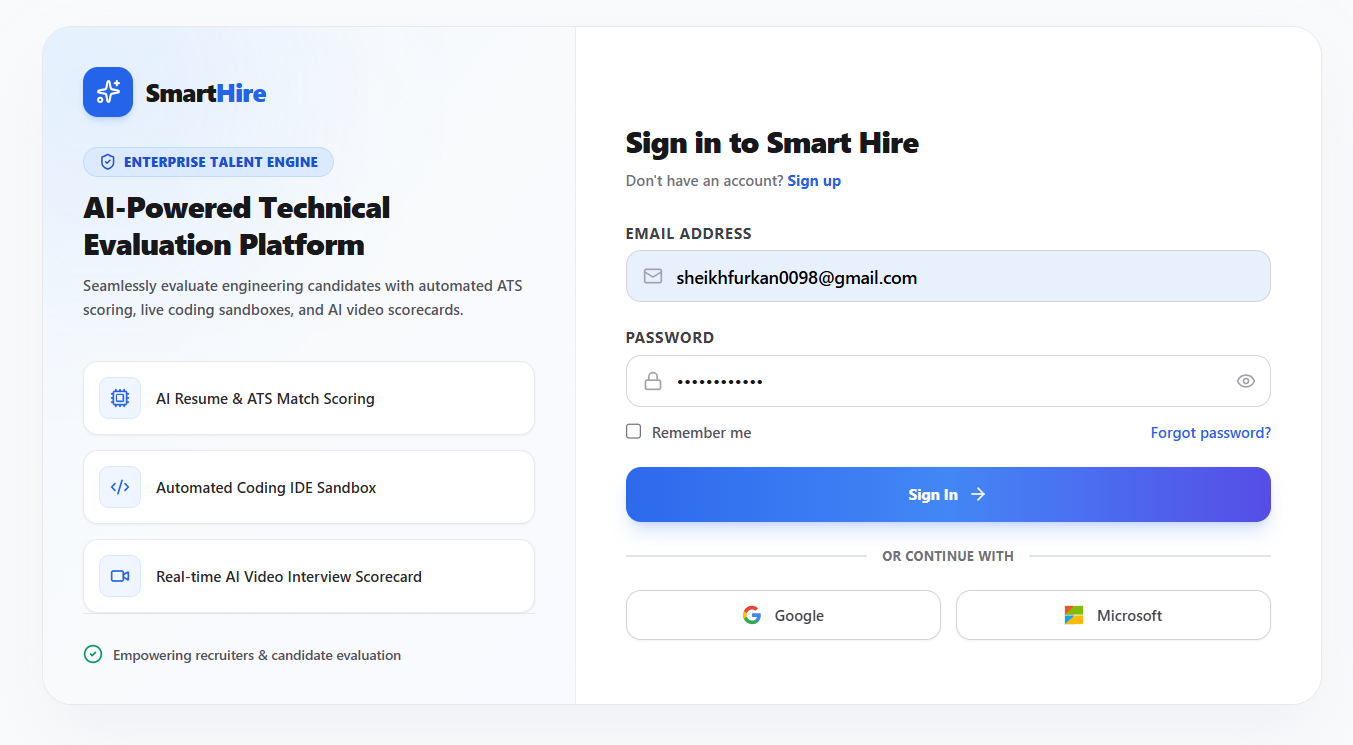
\includegraphics[width=0.85\textwidth]{images/login and registration interface.png}
  \caption{Login and registration interface}
  \label{fig:login_register}
\end{figure}

\subsection{Purpose}

The authentication module handles user registration, login, session token management, and role-based access control. It must distinguish between three user roles (candidate, recruiter, administrator) and route each user to the appropriate portal upon successful authentication.

\subsection{Implementation Details}

Authentication is delegated to Supabase Auth, which provides email/password registration, JWT token issuance, and session refresh. A critical implementation detail is the browser client singleton pattern. In a Next.js application, components may re-render frequently during hydration; creating a new Supabase client on each render would produce redundant network connections and potential race conditions. The singleton ensures that only one client instance exists per browser tab.

\begin{lstlisting}[language=Java, caption={Supabase browser client singleton}]
// apps/web/src/utils/supabase/client.ts
import { createBrowserClient } from "@supabase/ssr";

let browserClient: ReturnType<typeof createBrowserClient> | null
  = null;

export function getSupabaseBrowserClient() {
  if (typeof window === "undefined") {
    // SSR: create a fresh client per request
    return createBrowserClient(
      process.env.NEXT_PUBLIC_SUPABASE_URL!,
      process.env.NEXT_PUBLIC_SUPABASE_ANON_KEY!
    );
  }
  if (!browserClient) {
    browserClient = createBrowserClient(
      process.env.NEXT_PUBLIC_SUPABASE_URL!,
      process.env.NEXT_PUBLIC_SUPABASE_ANON_KEY!
    );
  }
  return browserClient;
}
\end{lstlisting}

The conditional check on \texttt{typeof window} ensures that server-side rendering (where \texttt{window} is undefined) always creates a fresh client, avoiding stale session data across different server requests.

\subsection{Security Considerations}

Passwords are hashed by Supabase using bcrypt with a configurable cost factor. JWT tokens are stored in HTTP-only cookies to prevent cross-site scripting (XSS) attacks from accessing them. API routes validate the JWT on every request using Supabase's \texttt{getUser()} method, which verifies the token signature and checks expiration.

\section{Module 2: Job Management}
\label{sec:impl-jobs}

\begin{figure}[H]
  \centering
  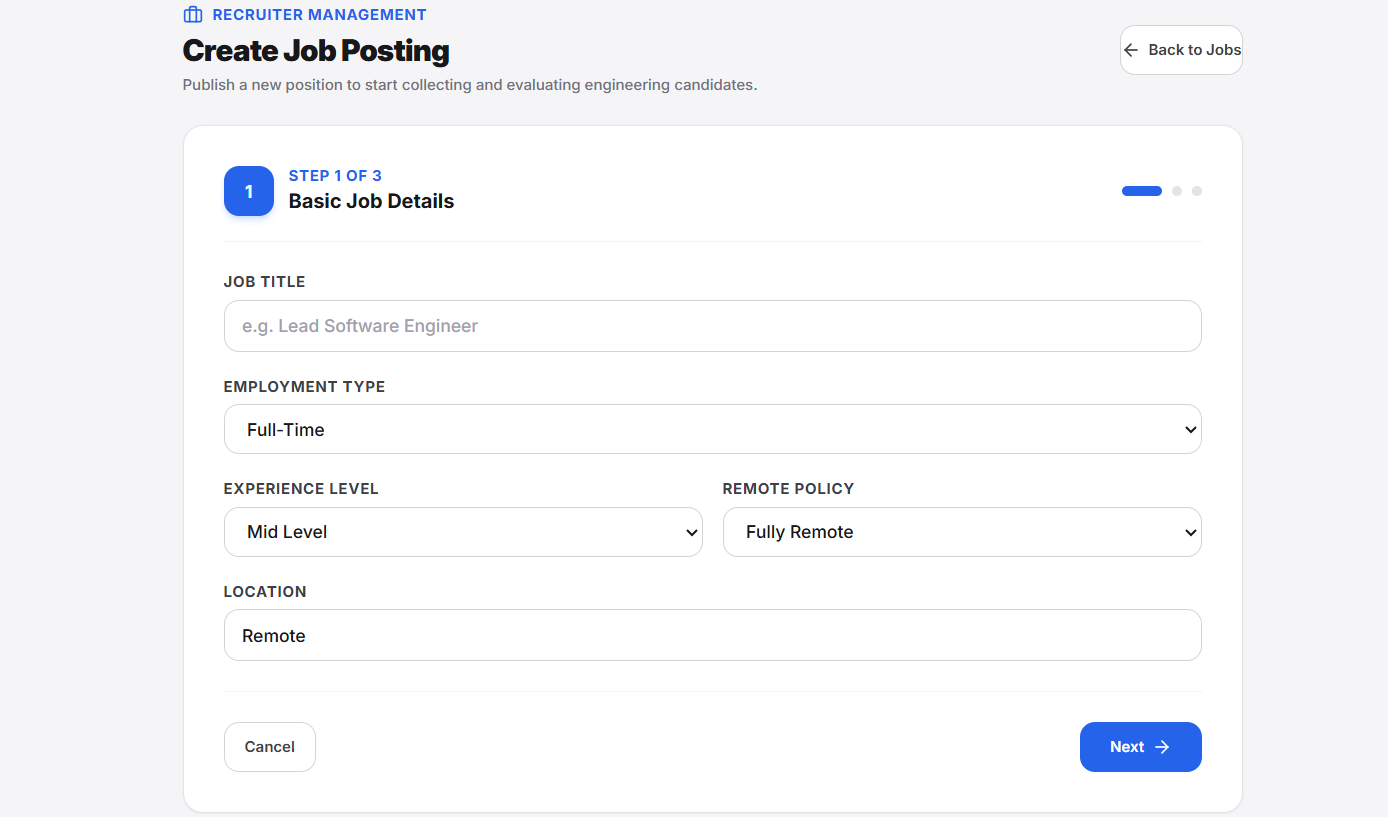
\includegraphics[width=0.85\textwidth]{images/job creation interface.png}
  \caption{Job creation wizard interface showcasing light mode theme and multi-step positioning parameters.}
  \label{fig:job_creation}
\end{figure}

\subsection{Purpose}

The job management module allows recruiters to create, edit, publish, and close job postings. Each job posting specifies a title, description, required skills, location, employment type, salary range, and a status field that governs visibility to candidates.

\subsection{Workflow}

Jobs follow a simple lifecycle: \textbf{Draft} $\rightarrow$ \textbf{Published} $\rightarrow$ \textbf{Closed}. A newly created job defaults to draft status and is not visible on the candidate portal. When the recruiter publishes the job, it appears in the public job directory. Closing a job removes it from the directory and prevents new applications.

\subsection{Database Interaction}

The job service (\texttt{job-service.ts}) exposes methods for creating, retrieving, updating, and listing jobs. All queries are scoped to the authenticated recruiter's company to enforce multi-tenant isolation:

\begin{lstlisting}[language=Java, caption={Job retrieval scoped to recruiter's company}]
async function getJobsByRecruiter(recruiterId: string) {
  const { data, error } = await supabase
    .from("job.jobs")
    .select("*")
    .eq("recruiter_id", recruiterId)
    .order("created_at", { ascending: false });
  if (error) throw error;
  return data;
}
\end{lstlisting}

\section{Module 3: Candidate Profile and Job Directory}
\label{sec:impl-candidate}

\begin{figure}[H]
  \centering
  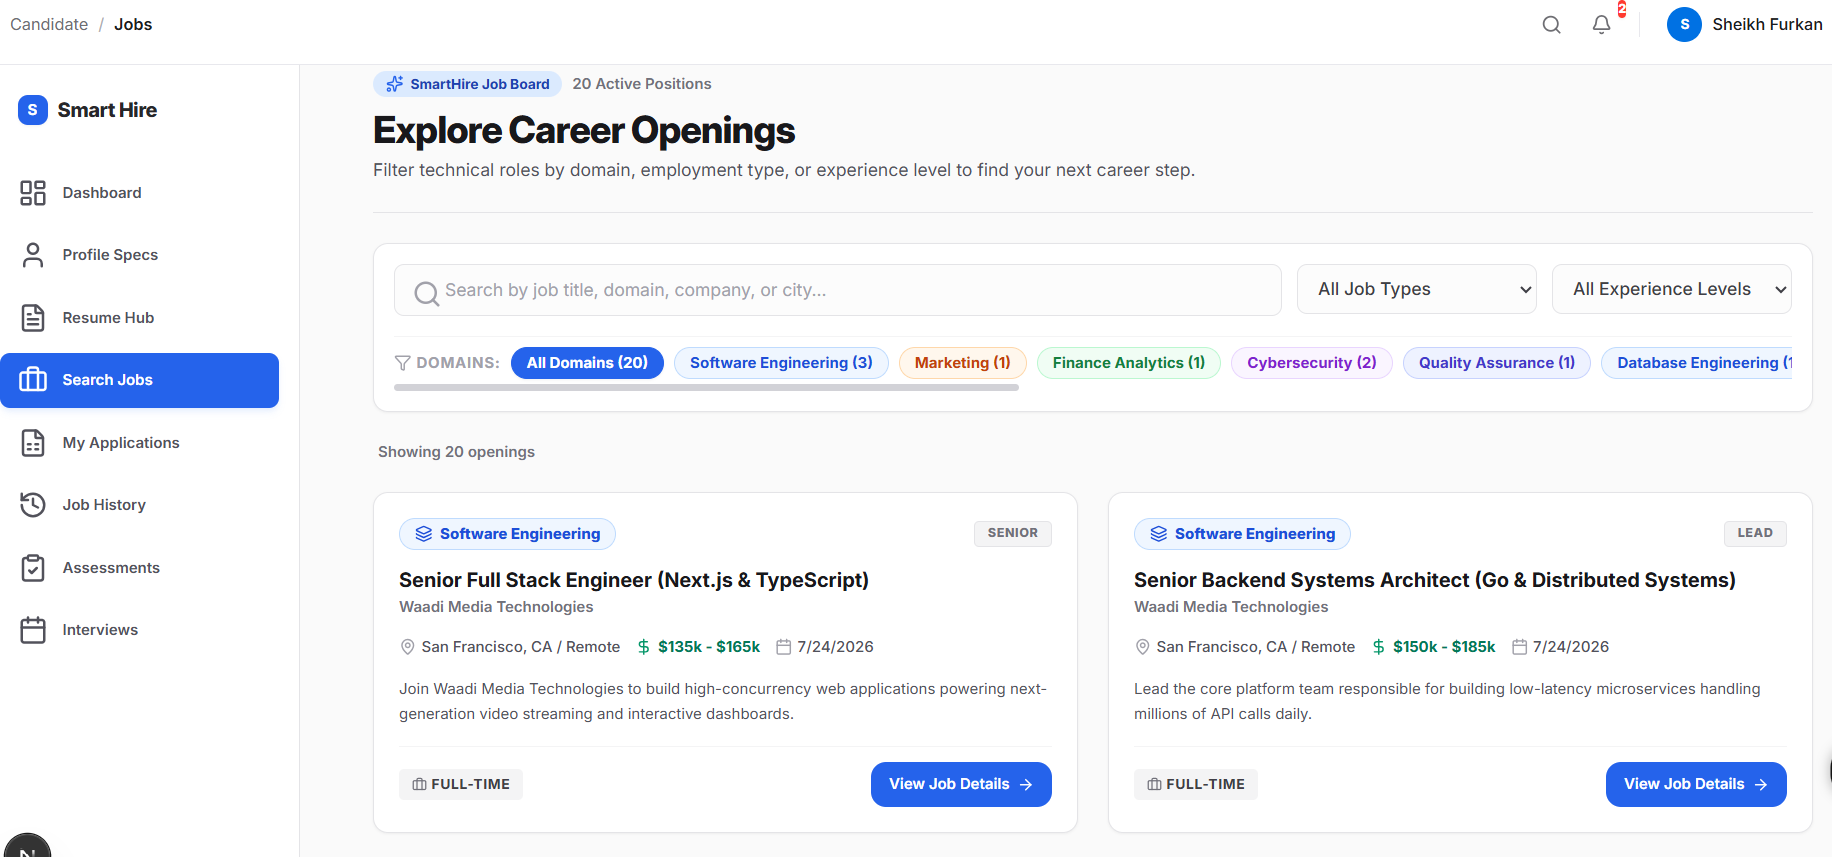
\includegraphics[width=0.85\textwidth]{images/candidate job dirwithsearchfilters.png}
  \caption{Candidate job directory with search filters}
  \label{fig:candidate_job_directory}
\end{figure}

\begin{figure}[H]
  \centering
  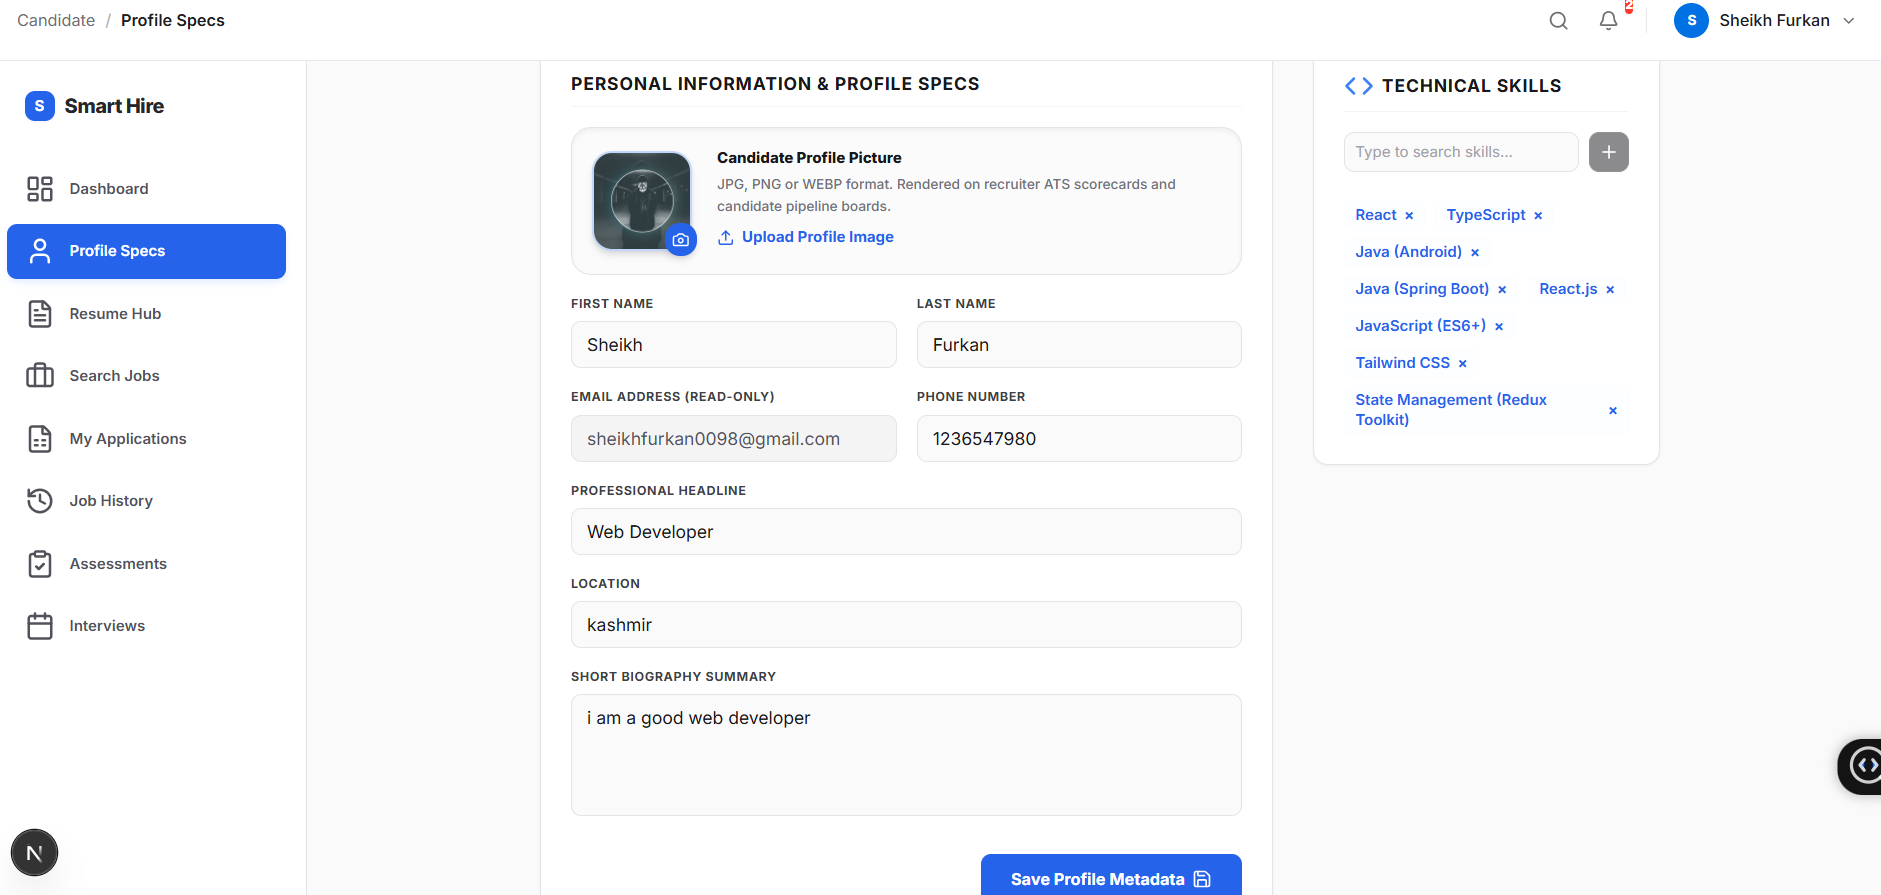
\includegraphics[width=0.85\textwidth]{images/candidate profile editor.png}
  \caption{Candidate profile editor interface}
  \label{fig:candidate_profile_editor}
\end{figure}

\subsection{Purpose}

Candidates need a profile that stores their personal information, skills, education, and work experience. They also need to browse and search published job listings.

\subsection{Implementation Details}

The candidate profile is pre-populated from Supabase Auth metadata (name, email) upon first login, reducing manual data entry. Additional fields (phone, skills array, experience years) are stored in the \texttt{candidate.candidates} table. The job directory page fetches all published jobs using a filtered query and presents them in a searchable, paginated grid. Candidates can filter by keyword, location, job category, and employment type.

\section{Module 4: Resume Upload and ATS Scoring}
\label{sec:impl-ats}

\begin{figure}[H]
  \centering
  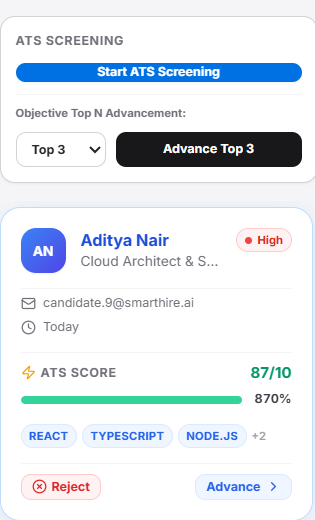
\includegraphics[width=0.65\textwidth]{images/ats view.png}
  \caption{ATS Board}
  \label{fig:ats_board}
\end{figure}

\subsection{Purpose}

When a candidate applies for a job, the system must extract text from the uploaded PDF resume, parse it into structured fields, and compute a relevance score against the job description.

\subsection{Workflow}

\begin{enumerate}[leftmargin=1.5em]
  \item The candidate selects a PDF file and submits the application form.
  \item The frontend uploads the file to Supabase Storage and sends the file URL along with the application data to the API.
  \item The resume service extracts text from the PDF using a server-side parsing library.
  \item The extracted text and the job description are sent to the Gemini API with a structured prompt requesting a relevance score on a 0--10 scale, along with dimensional breakdowns.
  \item The API response is parsed, validated, and stored in the application record.
\end{enumerate}

\section{Module 5: MCQ Assessment Engine}
\label{sec:impl-mcq}

\begin{figure}[H]
  \centering
  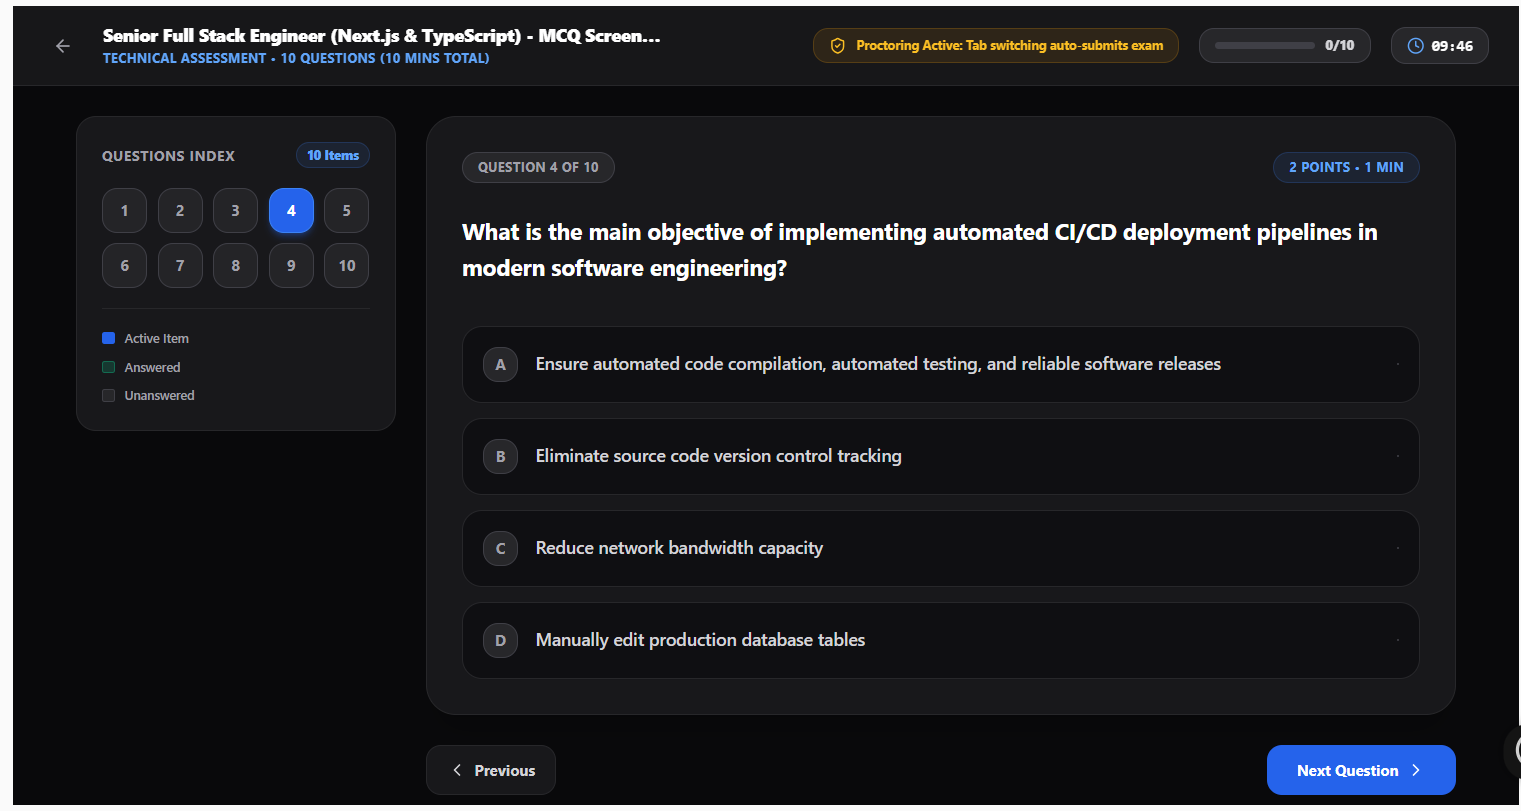
\includegraphics[width=0.85\textwidth]{images/mcq.png}
  \caption{MCQ examination interface with countdown timer}
  \label{fig:mcq_exam}
\end{figure}

\subsection{Purpose}

The MCQ engine administers timed multiple-choice assessments to candidates who pass the ATS screening threshold. It must enforce time limits, randomise question order to reduce cheating, auto-submit when the timer expires, and compute scores instantly.

\subsection{Implementation Details}

Each job can have an associated question pool stored in the \texttt{assessment.questions} table. When a candidate begins an MCQ assessment, the system creates an attempt record in \texttt{assessment.attempts}, selects questions from the pool, randomises their order, and starts a client-side countdown timer. The timer is implemented using React's \texttt{useEffect} hook with a one-second interval. If the timer reaches zero before the candidate manually submits, the system automatically submits all recorded answers.

Score computation is straightforward: the number of correct answers divided by the total number of questions, multiplied by 100. The computed score is stored in the application record.

\section{Module 6: Interactive Coding Assessment}
\label{sec:impl-coding}

\begin{figure}[H]
  \centering
  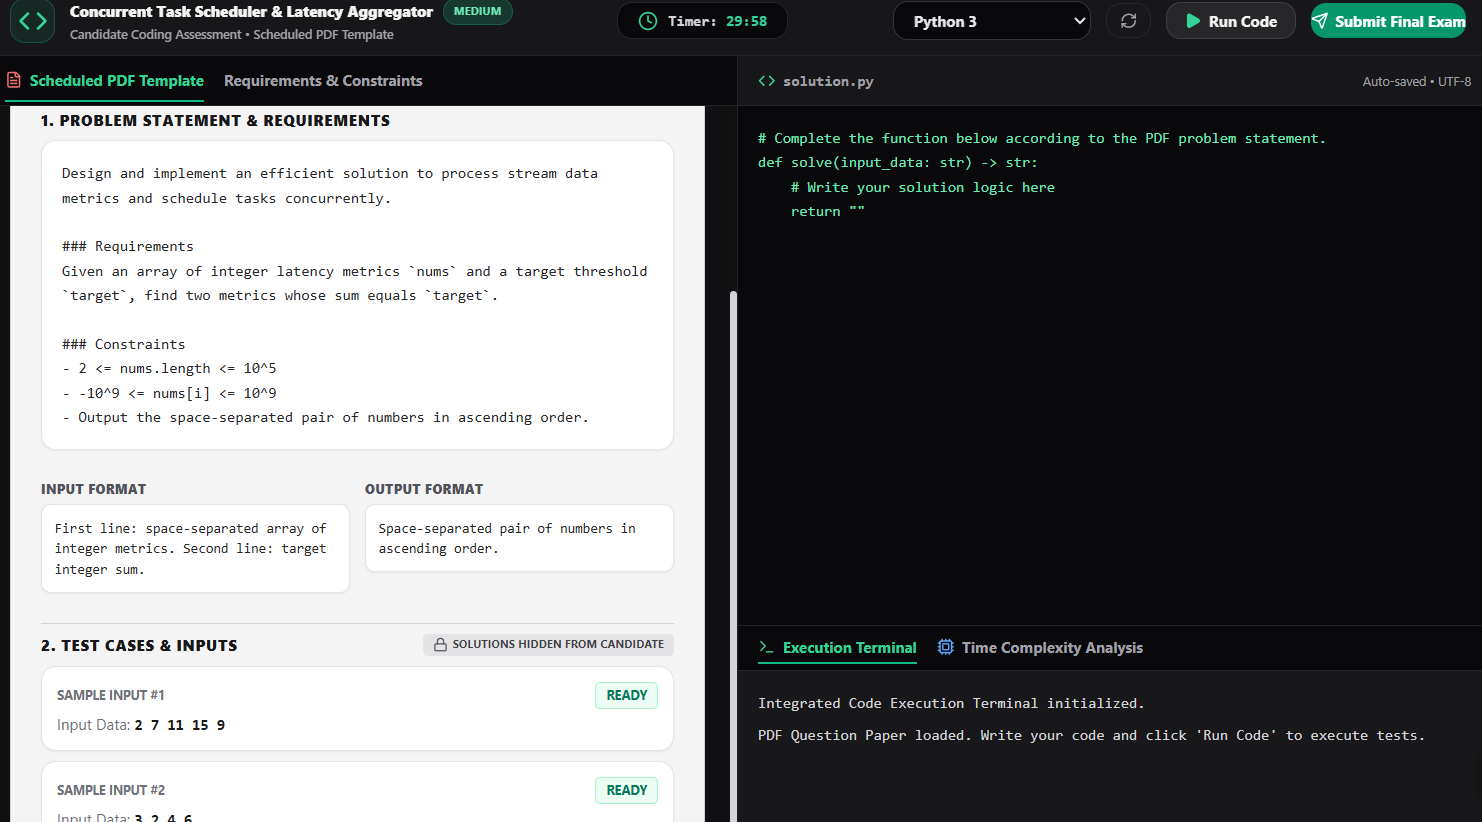
\includegraphics[width=0.85\textwidth]{images/coding round.png}
  \caption{coding round ide}
  \label{fig:coding_ide}
\end{figure}

\subsection{Purpose}

The coding module provides a browser-based IDE where candidates write and execute code to solve programming challenges. It replaces the need for a separate coding assessment platform.

\subsection{Implementation Details}

The code editor is built using \texttt{@monaco-editor/react}, which embeds the same editing engine used by Visual Studio Code. The editor supports syntax highlighting, auto-indentation, and bracket matching for JavaScript and Python. When the candidate clicks ``Run,'' the code is sent to a server-side API endpoint that executes it in a sandboxed environment, captures the output, and compares it against expected results for each test case.

Each test case specifies an input string and an expected output string. The execution environment runs the candidate's code with the input piped to stdin, captures stdout, and performs a string comparison. Test results are returned to the frontend, showing pass/fail status for each test case. The final score is the percentage of test cases passed.

\section{Module 7: AI Video Interview}
\label{sec:impl-interview}

\begin{figure}[H]
  \centering
  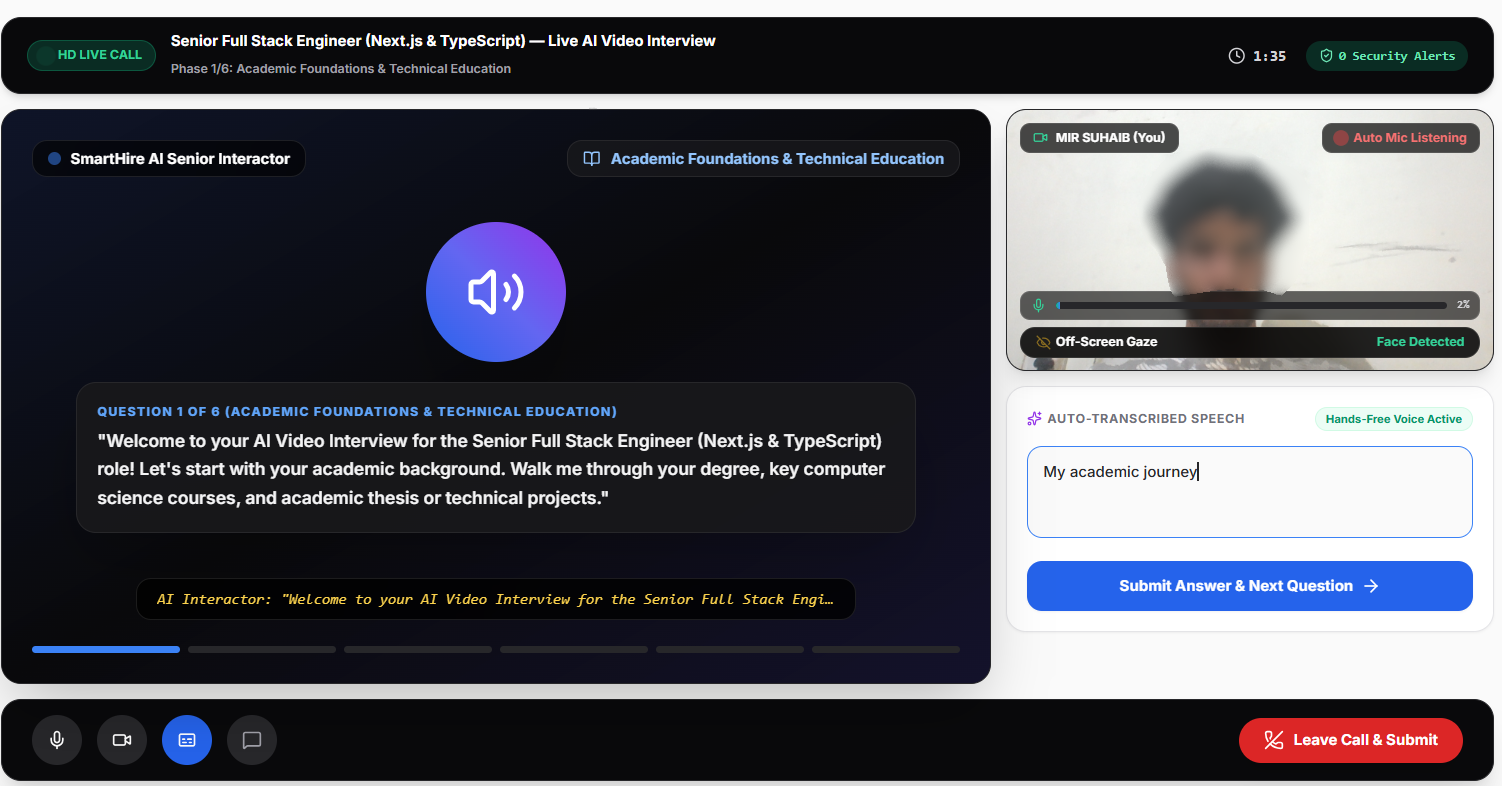
\includegraphics[width=0.85\textwidth]{images/ai interview.png}
  \caption{Live AI video interview recording room with real-time audio transcript, proctoring gaze detection, and voice evaluation.}
  \label{fig:ai_interview}
\end{figure}

\subsection{Purpose}

The video interview module enables asynchronous, AI-evaluated interviews. Candidates record responses to predefined questions, and the system uses the Gemini API to evaluate the quality of their answers.

\subsection{Implementation Details}

The interview interface presents questions one at a time. For each question, the candidate clicks ``Record,'' speaks their response while being recorded via the browser's MediaRecorder API, and clicks ``Stop'' when finished. The recorded audio is transcribed (either client-side using the Web Speech API or server-side using a transcription service) and stored alongside the question in a structured format.

Once all questions have been answered, the complete set of question-response pairs is sent to the Gemini API with an evaluation prompt. The prompt instructs the model to assess each response across four dimensions: \textit{technical knowledge}, \textit{communication clarity}, \textit{problem-solving approach}, and \textit{depth of reasoning}. The model returns a structured JSON scorecard with per-dimension ratings and an overall recommendation.

\subsection{Scorecard Categories}

The overall recommendation uses a five-point scale:

\begin{table}[htbp]
\centering
\caption{AI interview scorecard recommendation categories}
\label{tab:scorecard}
\small
\begin{tabular}{lp{4in}}
\toprule
\textbf{Category} & \textbf{Interpretation} \\
\midrule
\texttt{strong\_hire}    & Exceptional responses; candidate demonstrates deep expertise and clear communication. \\
\texttt{hire}            & Solid responses; candidate meets or exceeds expectations. \\
\texttt{neutral}         & Adequate responses; further evaluation may be warranted. \\
\texttt{no\_hire}         & Below expectations; significant gaps in knowledge or communication. \\
\texttt{strong\_no\_hire}  & Poor responses; candidate does not meet minimum requirements. \\
\bottomrule
\end{tabular}
\end{table}

\section{Module 8: Recruiter Kanban Pipeline}
\label{sec:impl-kanban}

\begin{figure}[H]
  \centering
  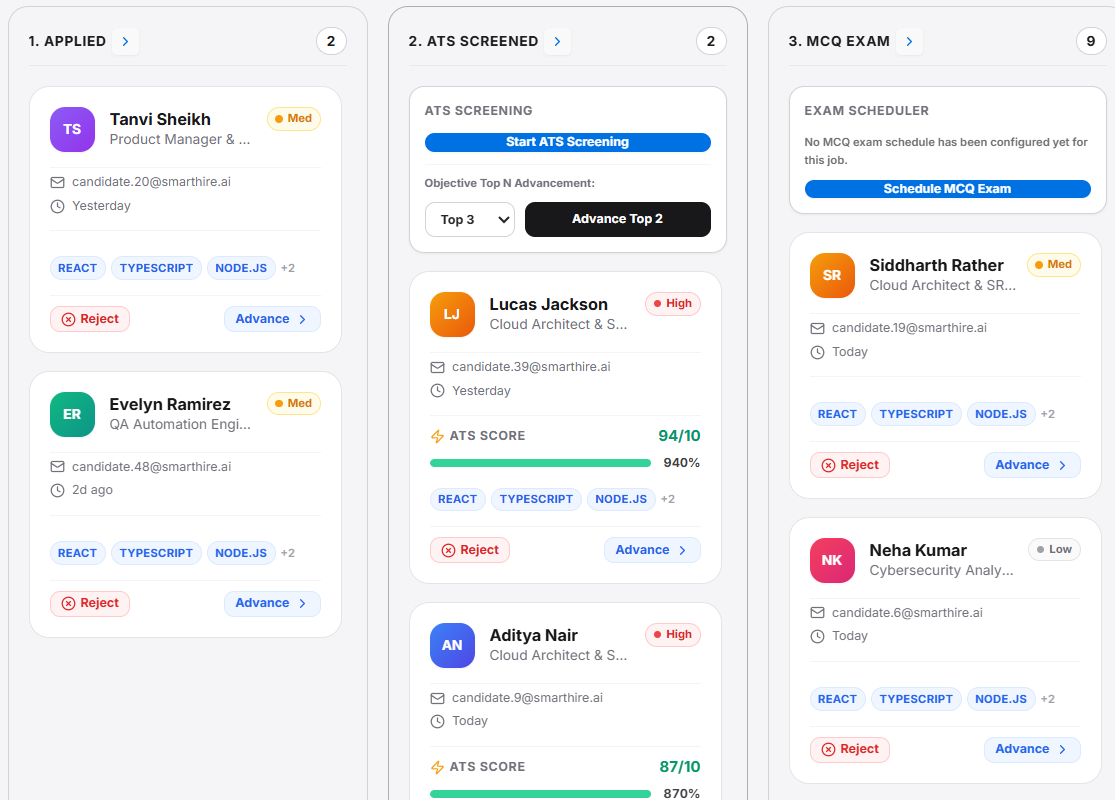
\includegraphics[width=0.85\textwidth]{images/kanban board.png}
  \caption{Recruiter Kanban pipeline board showing multi-stage candidate progression and automated ATS screening controls.}
  \label{fig:pipeline_board}
\end{figure}

\subsection{Purpose}

The Kanban board gives recruiters a visual overview of all candidates for a given job, organised by pipeline stage. It supports drag-and-drop stage transitions, real-time status updates, and stage-specific rejection tracking.

\subsection{Implementation Details}

The Kanban board is implemented as a client-side React component that fetches all applications for the selected job and groups them into columns by stage. Each column represents a pipeline stage: Applied, ATS Screened, MCQ, Coding, Interview, Offer, and Hired. Dragging a card from one column to another triggers an API call that updates the application's stage in the database.

Stage transitions are validated on the server to ensure they follow the prescribed order. If a recruiter moves a candidate to a rejected state, the system records which stage the rejection occurred at and optionally logs a rejection reason. This information is surfaced on the candidate's application history page.

\section{Module 9: Recruiter Dashboard}
\label{sec:impl-dashboard}

\begin{figure}[H]
  \centering
  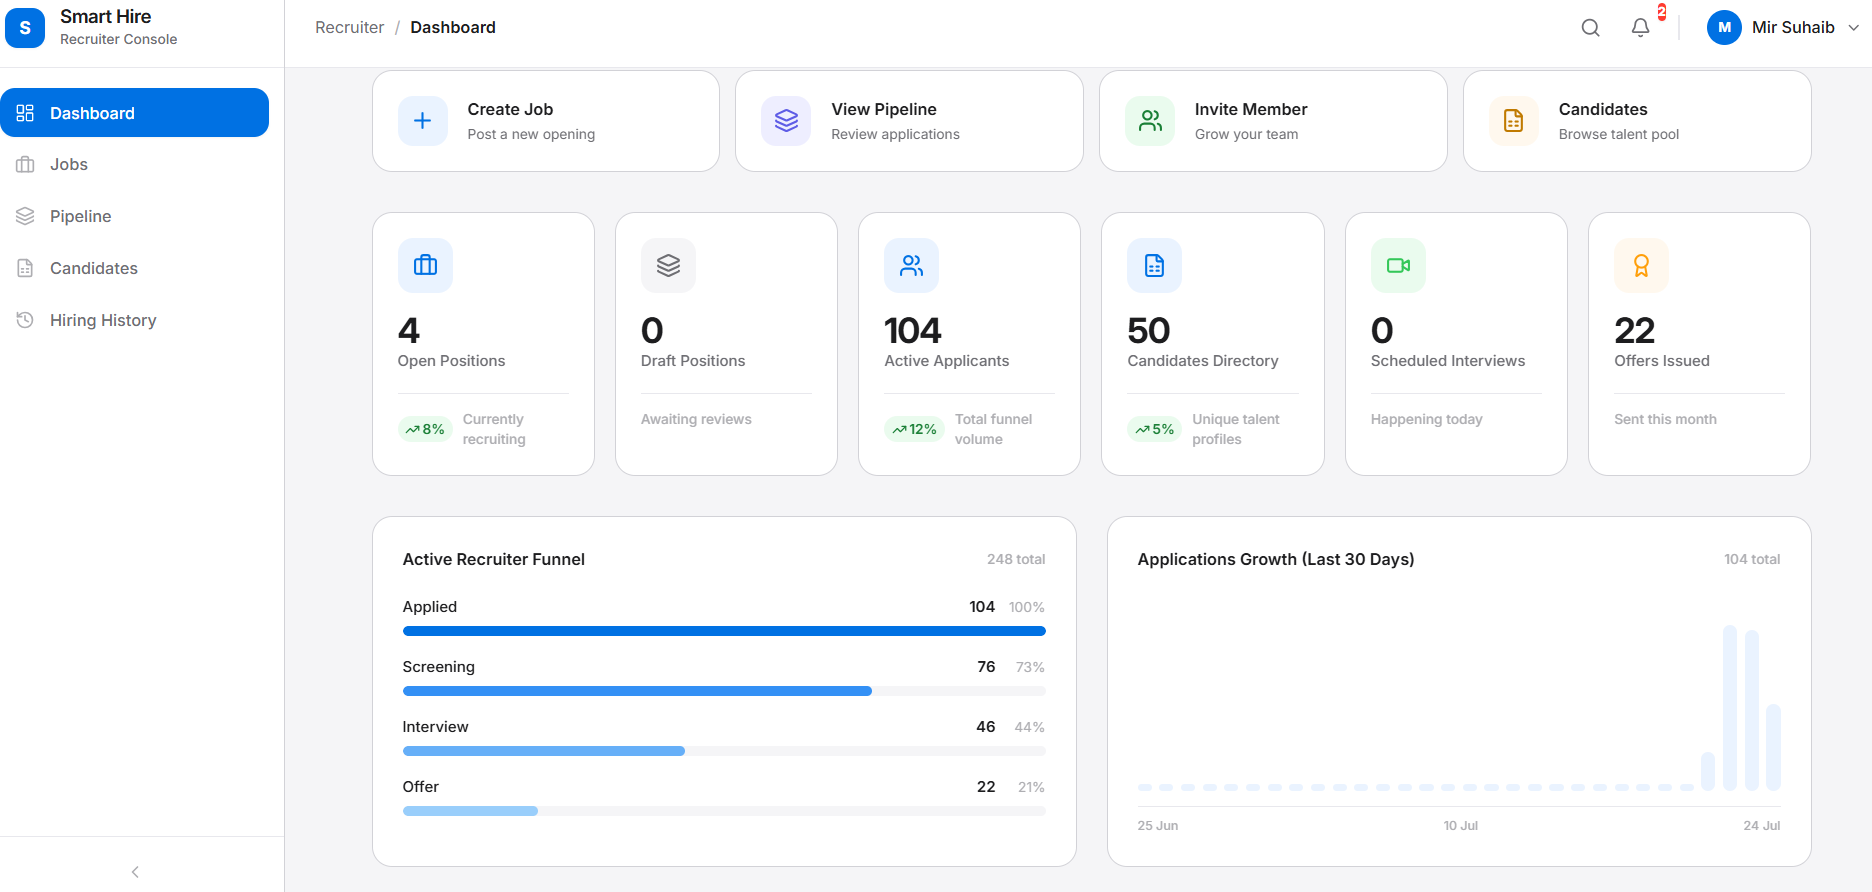
\includegraphics[width=0.85\textwidth]{images/recruiter dasboard with hiring metrics.png}
  \caption{Recruiter dashboard displaying real-time hiring funnel metrics, active applicant counts, and application growth analytics.}
  \label{fig:recruiter_dashboard}
\end{figure}

\subsection{Purpose}

The dashboard provides recruiters with at-a-glance metrics on their hiring activity: open positions, active applicants, interviews scheduled, offers issued, and pipeline funnel analytics.

\subsection{Multi-Tenant Scoping}

A critical design requirement is that each recruiter sees only metrics related to their own job postings. The dashboard queries are scoped by joining the \texttt{application.applications} table against the \texttt{job.jobs} table where the \texttt{recruiter\_id} matches the authenticated user. This prevents data from other recruiters (even within the same company) from leaking into the dashboard view.

\section{Module 10: Offer Letter Generation}
\label{sec:impl-offer}

\begin{figure}[H]
  \centering
  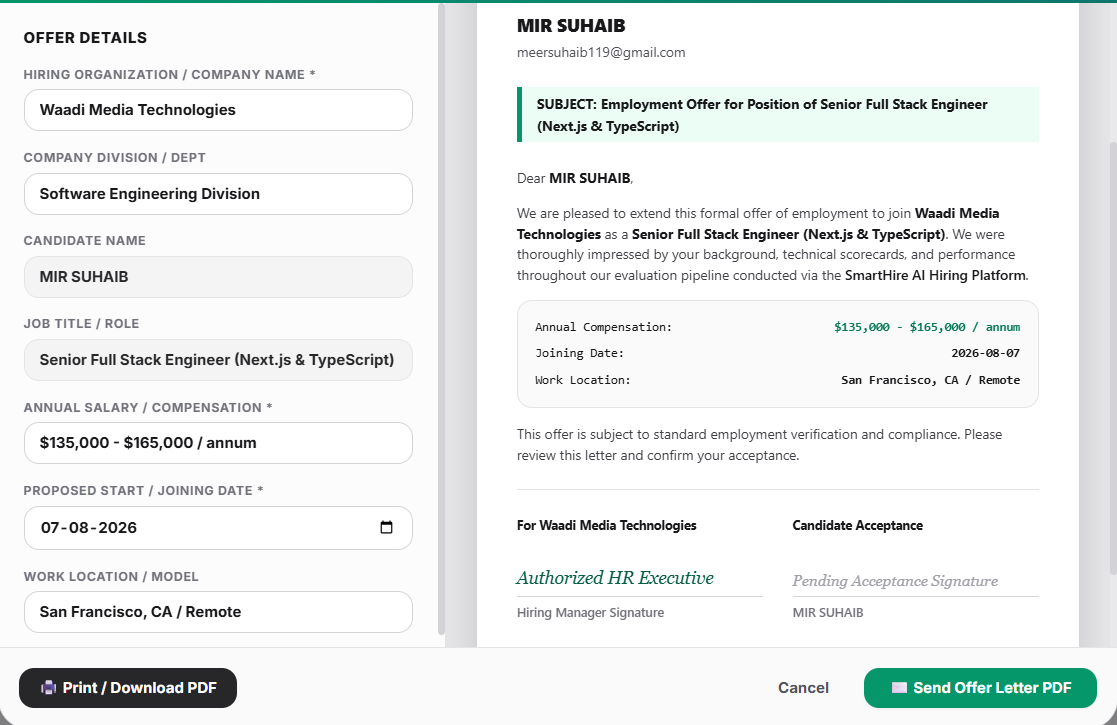
\includegraphics[width=0.85\textwidth]{images/offerletter.png}
  \caption{Official offer letter generator interface with real-time PDF preview and signature workflow.}
  \label{fig:offer_letter}
\end{figure}

\subsection{Purpose}

Once a recruiter decides to hire a candidate, the system generates a formal PDF offer letter that can be customised, previewed, and dispatched to the candidate.

\subsection{Implementation Details}

Offer letters are generated client-side using the jsPDF library combined with html2canvas for rendering styled HTML templates into PDF format. The recruiter fills in a form specifying salary, joining date, position title, and any special terms. The system renders a preview of the offer letter in the browser, and the recruiter can download the PDF or send it directly to the candidate through the platform.

When the candidate receives an offer, they see it on their application history page and can accept or decline it. The acceptance status is recorded in the database and reflected on the recruiter's Kanban board.

\section{Module 11: Responsive Navigation}
\label{sec:impl-nav}

\begin{figure}[H]
  \centering
  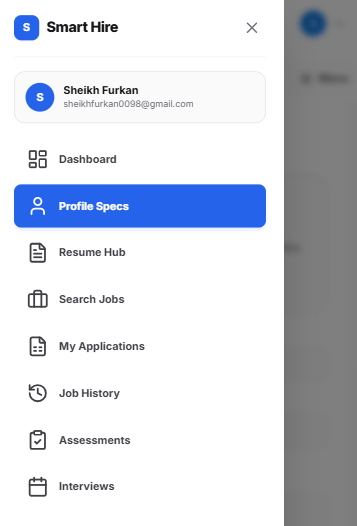
\includegraphics[width=0.50\textwidth]{images/mobile navigation drawer.png}
  \caption{Mobile responsive navigation drawer}
  \label{fig:mobile_drawer}
\end{figure}

The platform provides distinct navigation experiences for desktop and mobile viewports. On desktop, a persistent sidebar provides access to all portal sections. On mobile (viewport width below 768 pixels), the sidebar collapses into a hamburger menu that opens a slide-out drawer. Navigation state is managed using React's \texttt{useState} hook, and transitions are animated using CSS transforms for smooth visual feedback.

\section{Error Handling and Resilience Patterns}
\label{sec:impl-errors}

Robust error handling is essential for a production-grade application. SmartHire implements a layered error handling strategy that addresses failures at the network, API, database, and UI levels.

\subsection{API-Level Error Handling}

Every API route handler is wrapped in a try-catch block that catches both expected validation errors and unexpected runtime exceptions. Expected errors (invalid input, missing fields, unauthorised access) are returned with appropriate HTTP status codes and structured error messages. Unexpected errors are logged to the server console with full stack traces and returned to the client as generic 500 Internal Server Error responses to avoid leaking implementation details.

\begin{lstlisting}[language=Java, caption={Standardised API error handling pattern}]
export async function POST(request: NextRequest) {
  try {
    const body = await request.json();
    const validated = schema.parse(body); // throws on invalid
    const result = await service.process(validated);
    return NextResponse.json(result, { status: 201 });
  } catch (error) {
    if (error instanceof ZodError) {
      return NextResponse.json(
        { error: "Validation failed", details: error.issues },
        { status: 400 }
      );
    }
    console.error("Unexpected error:", error);
    return NextResponse.json(
      { error: "Internal server error" },
      { status: 500 }
    );
  }
}
\end{lstlisting}

\subsection{Client-Side Error Boundaries}

On the frontend, React error boundaries catch rendering errors in component subtrees and display fallback UI rather than crashing the entire page. Toast notifications are used to inform users of transient errors (network failures, API timeouts) without disrupting their workflow.

\subsection{External API Resilience}

Calls to the Gemini API are wrapped in a retry mechanism with exponential backoff. If the first request fails due to a transient network error or rate limit, the system waits for a brief interval before retrying, up to a maximum of three attempts. If all retries fail, the operation is marked as pending and the recruiter is notified that the AI evaluation could not be completed.

\section{Gemini API Integration Architecture}
\label{sec:impl-gemini}

The Gemini API integration is centralised in the \texttt{services/ai/} directory, which contains separate modules for resume evaluation and interview evaluation. Each module constructs a structured prompt, sends it to the Gemini API via an HTTPS POST request, parses the JSON response, validates the returned data against expected schemas, and stores the results.

\subsection{Prompt Template Management}

Prompt templates are stored as string constants within the service modules rather than in the database, allowing version-controlled iteration. Each template includes explicit instructions for the output format (JSON), the scoring dimensions, and the numeric scale. This structured approach ensures that the AI's output is machine-parseable and can be directly stored in the database without manual transformation.

\subsection{Response Validation}

AI model outputs are inherently non-deterministic. The integration layer validates every response against a schema that specifies required fields, numeric ranges, and allowed enumeration values. Responses that fail validation are logged for debugging and the operation is retried with a slightly modified prompt (e.g., adding a reminder about the expected output format). This defence-in-depth approach ensures that malformed AI responses never corrupt the application's data.

\section{Analytics and Reporting Module}
\label{sec:impl-analytics}

The analytics module aggregates data from across the platform to provide both recruiter-level and platform-level insights.

\subsection{Recruiter-Level Analytics}

Each recruiter's dashboard displays five key metrics, all scoped to the recruiter's own job postings:

\begin{itemize}[leftmargin=1.5em]
  \item \textbf{Open Positions}: Count of jobs with \texttt{status = 'published'}.
  \item \textbf{Active Applicants}: Count of applications with \texttt{status = 'active'} across the recruiter's jobs.
  \item \textbf{Interviews Scheduled}: Count of applications currently in the interview stage.
  \item \textbf{Offers Issued}: Count of applications that have reached the offer stage.
  \item \textbf{Hiring Funnel}: A breakdown showing how many candidates are at each pipeline stage, enabling the recruiter to identify bottlenecks.
\end{itemize}

\subsection{Platform-Level Analytics}

The administrator dashboard aggregates metrics across all tenants: total registered users (by role), total applications submitted, total jobs posted, and overall hiring funnel conversion rates. These metrics help platform operators monitor system utilisation and identify trends.

\subsection{Implementation Approach}

Analytics queries use PostgreSQL aggregate functions (\texttt{COUNT}, \texttt{GROUP BY}) with appropriate join conditions to compute metrics efficiently. Queries are executed on demand when the dashboard page loads rather than pre-computed, which simplifies the architecture at the cost of slightly higher query latency. For the current scale of the platform (hundreds of users, thousands of applications), on-demand computation is well within acceptable performance bounds.

